\begin{fact} \label{iso-tri}
	Considérons tous les triangles de périmètre fixé $p$. Parmi tous ces triangles, un seul est d'aire maximale, c'est le triangle équilatéral de côté $c = \dfrac13 p$.
\end{fact}


\begin{proof}	
	L'idée est la suivante: nous allons démontrer qu'une application itérative du fait \ref{tri-one-side-fixed} donne à la limite le triangle équilatéral d'aire maximale, et ceci avec une vitesse de convergence exponentielle.%
	\footnote{
		Ceci ne va nécessiter que l'emploi de propriétés simples de l'ensemble des réels.
	}
	Partons donc d'un triangle $ABC$ quelconque, mais de périmètre $p$, le fait \ref{tri-one-side-fixed} nous donne successivement les triangles $ACD$, $ADE$ et $AEF$ isocèles en $D$, $E$ et $F$ respectivement, ayant tous pour périmètre $p$, et ceci avec des aires de plus en plus grandes.  
	Le dessin suivant amène à conjecturer qu'en poursuivant le procédé pour avoir ensuite un triangle $AFG$ isocèle en $G$...\,, nous aboutirons \og \emph{à la limite} \fg\ à un triangle équilatéral.

	\begin{center}
		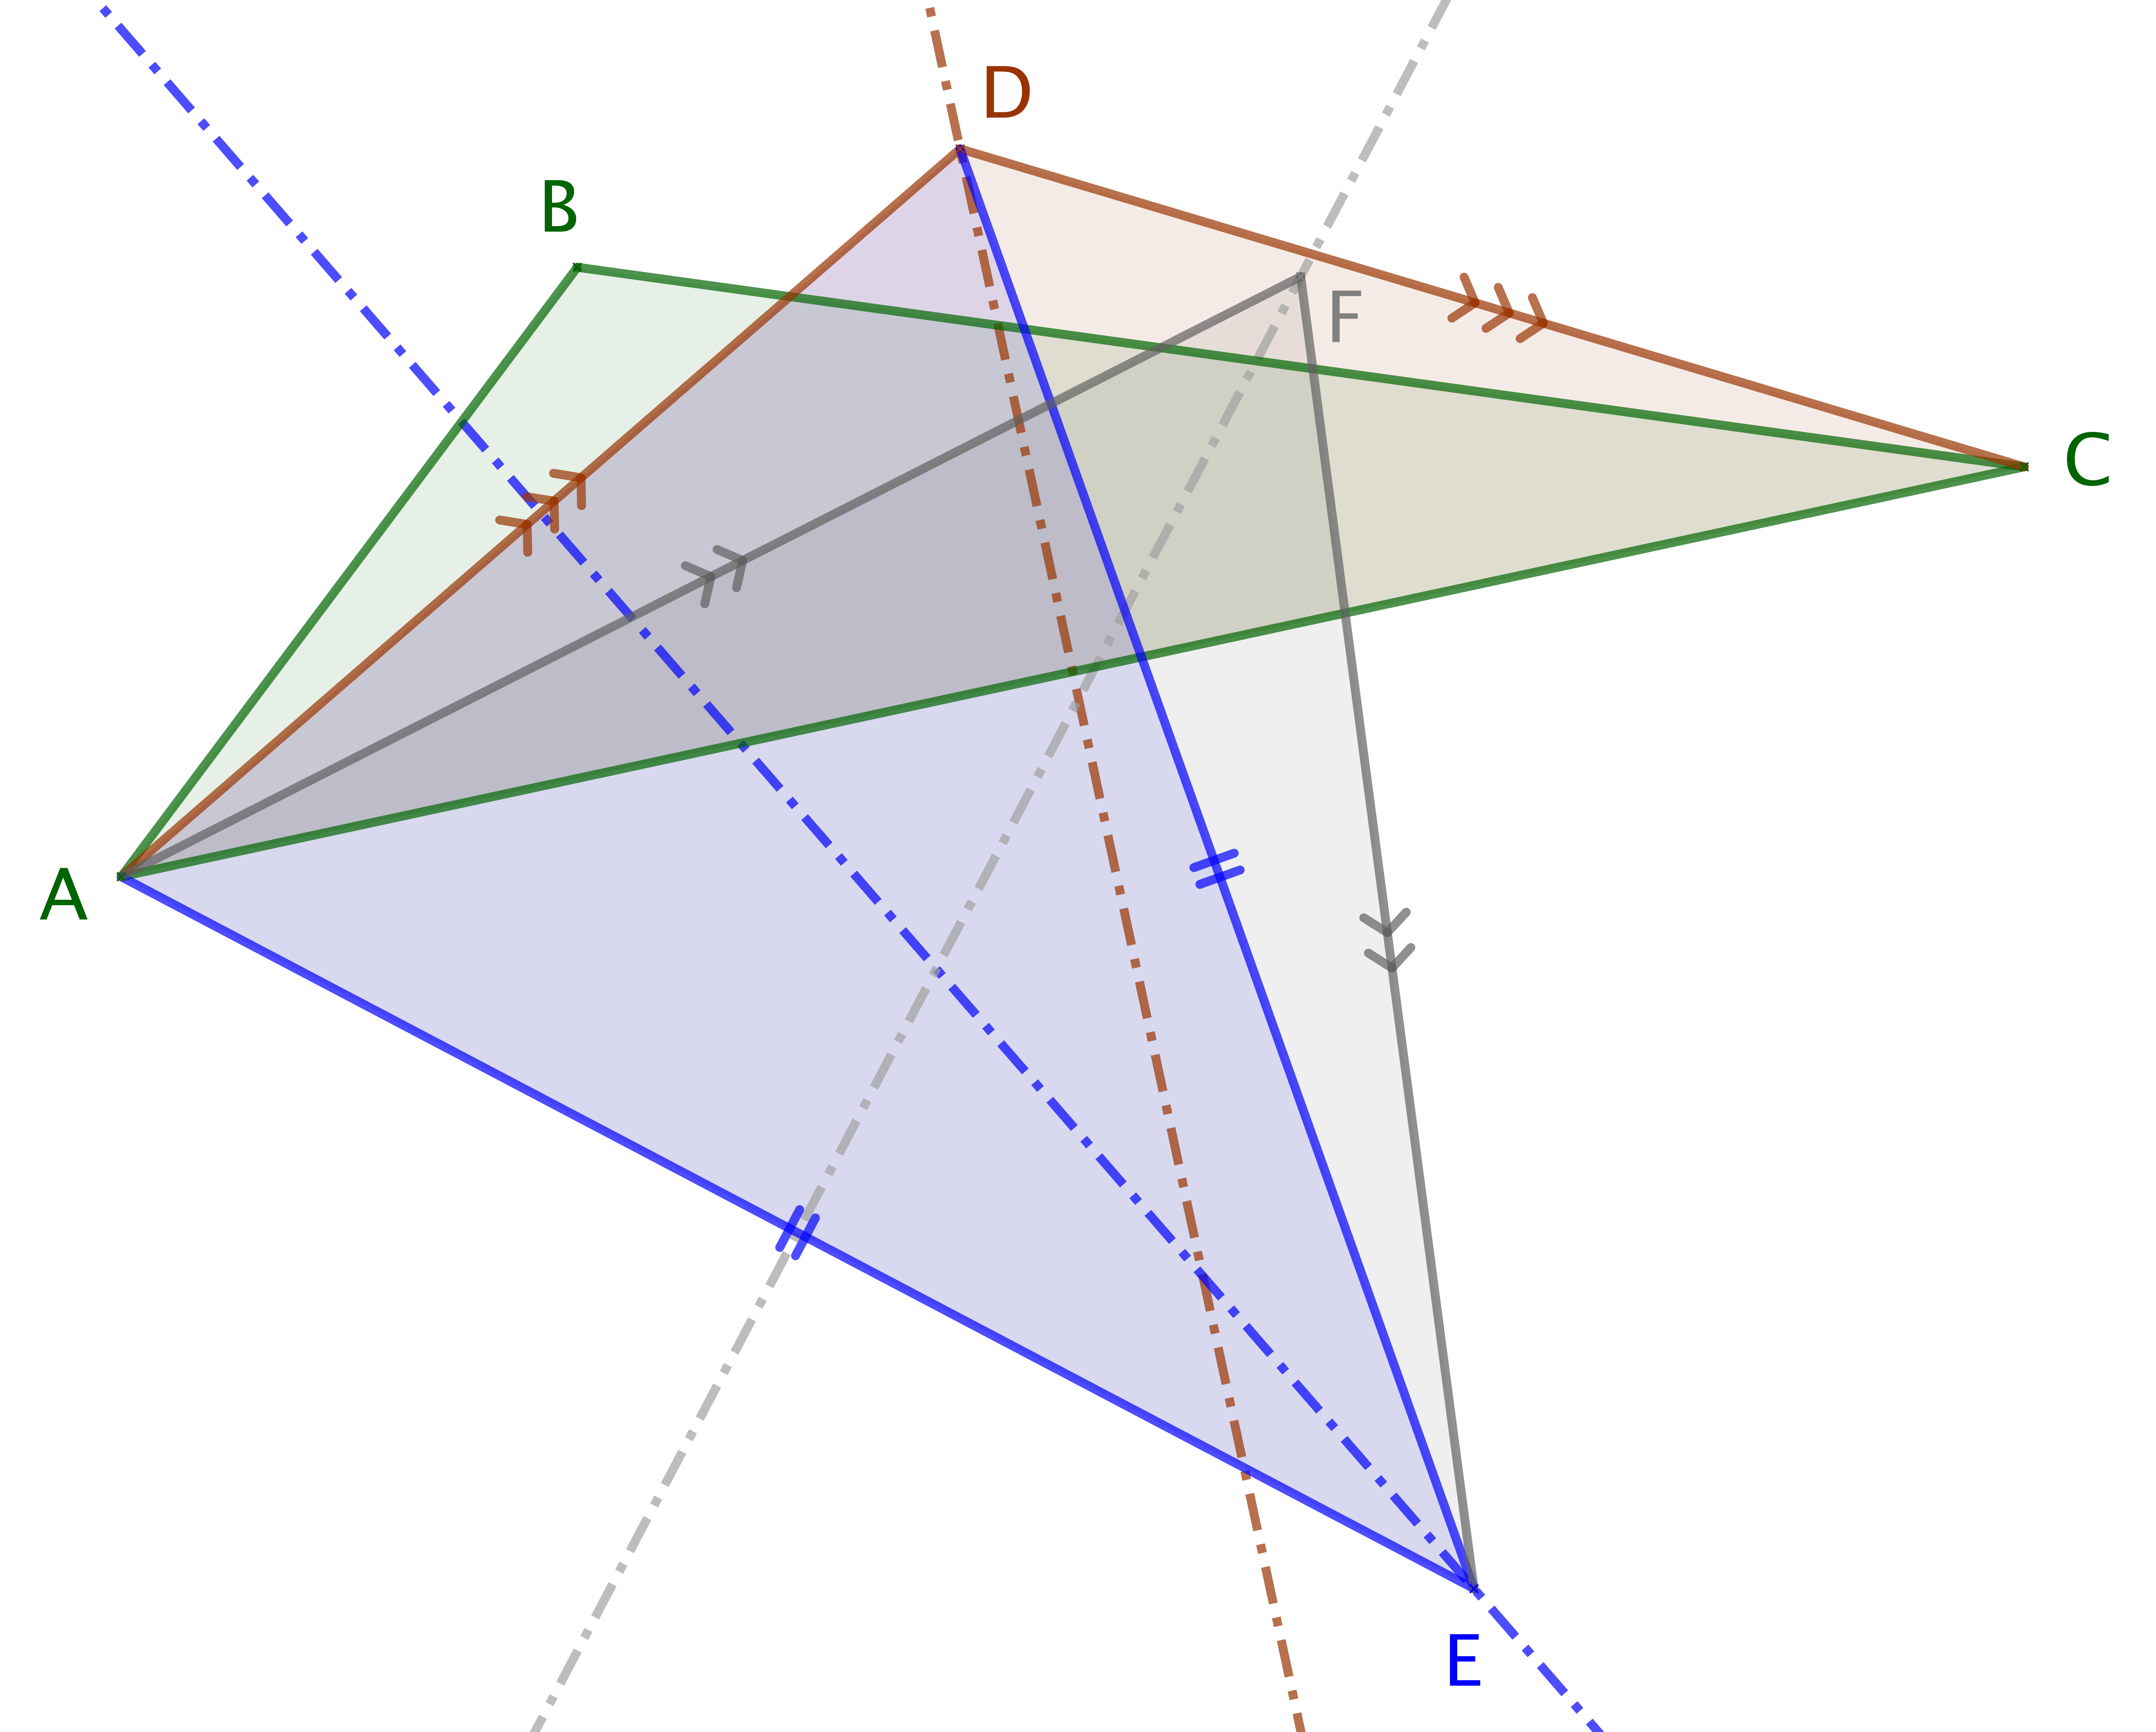
\includegraphics[scale=.4]{content/triangle-gene/triangle-conj.png}
	\end{center} 

	
	Le passage d'un triangle quelconque $ABC$ au triangle $ACD$ isocèle en $D$ nous amène à nous concentrer sur ce que donne notre procédé d'agrandissement d'aire à périmètre fixé pour des triangles isocèles. 
	Dans la suite, nous allons nous appuyer sur le schéma suivant.
	
	\begin{center}
		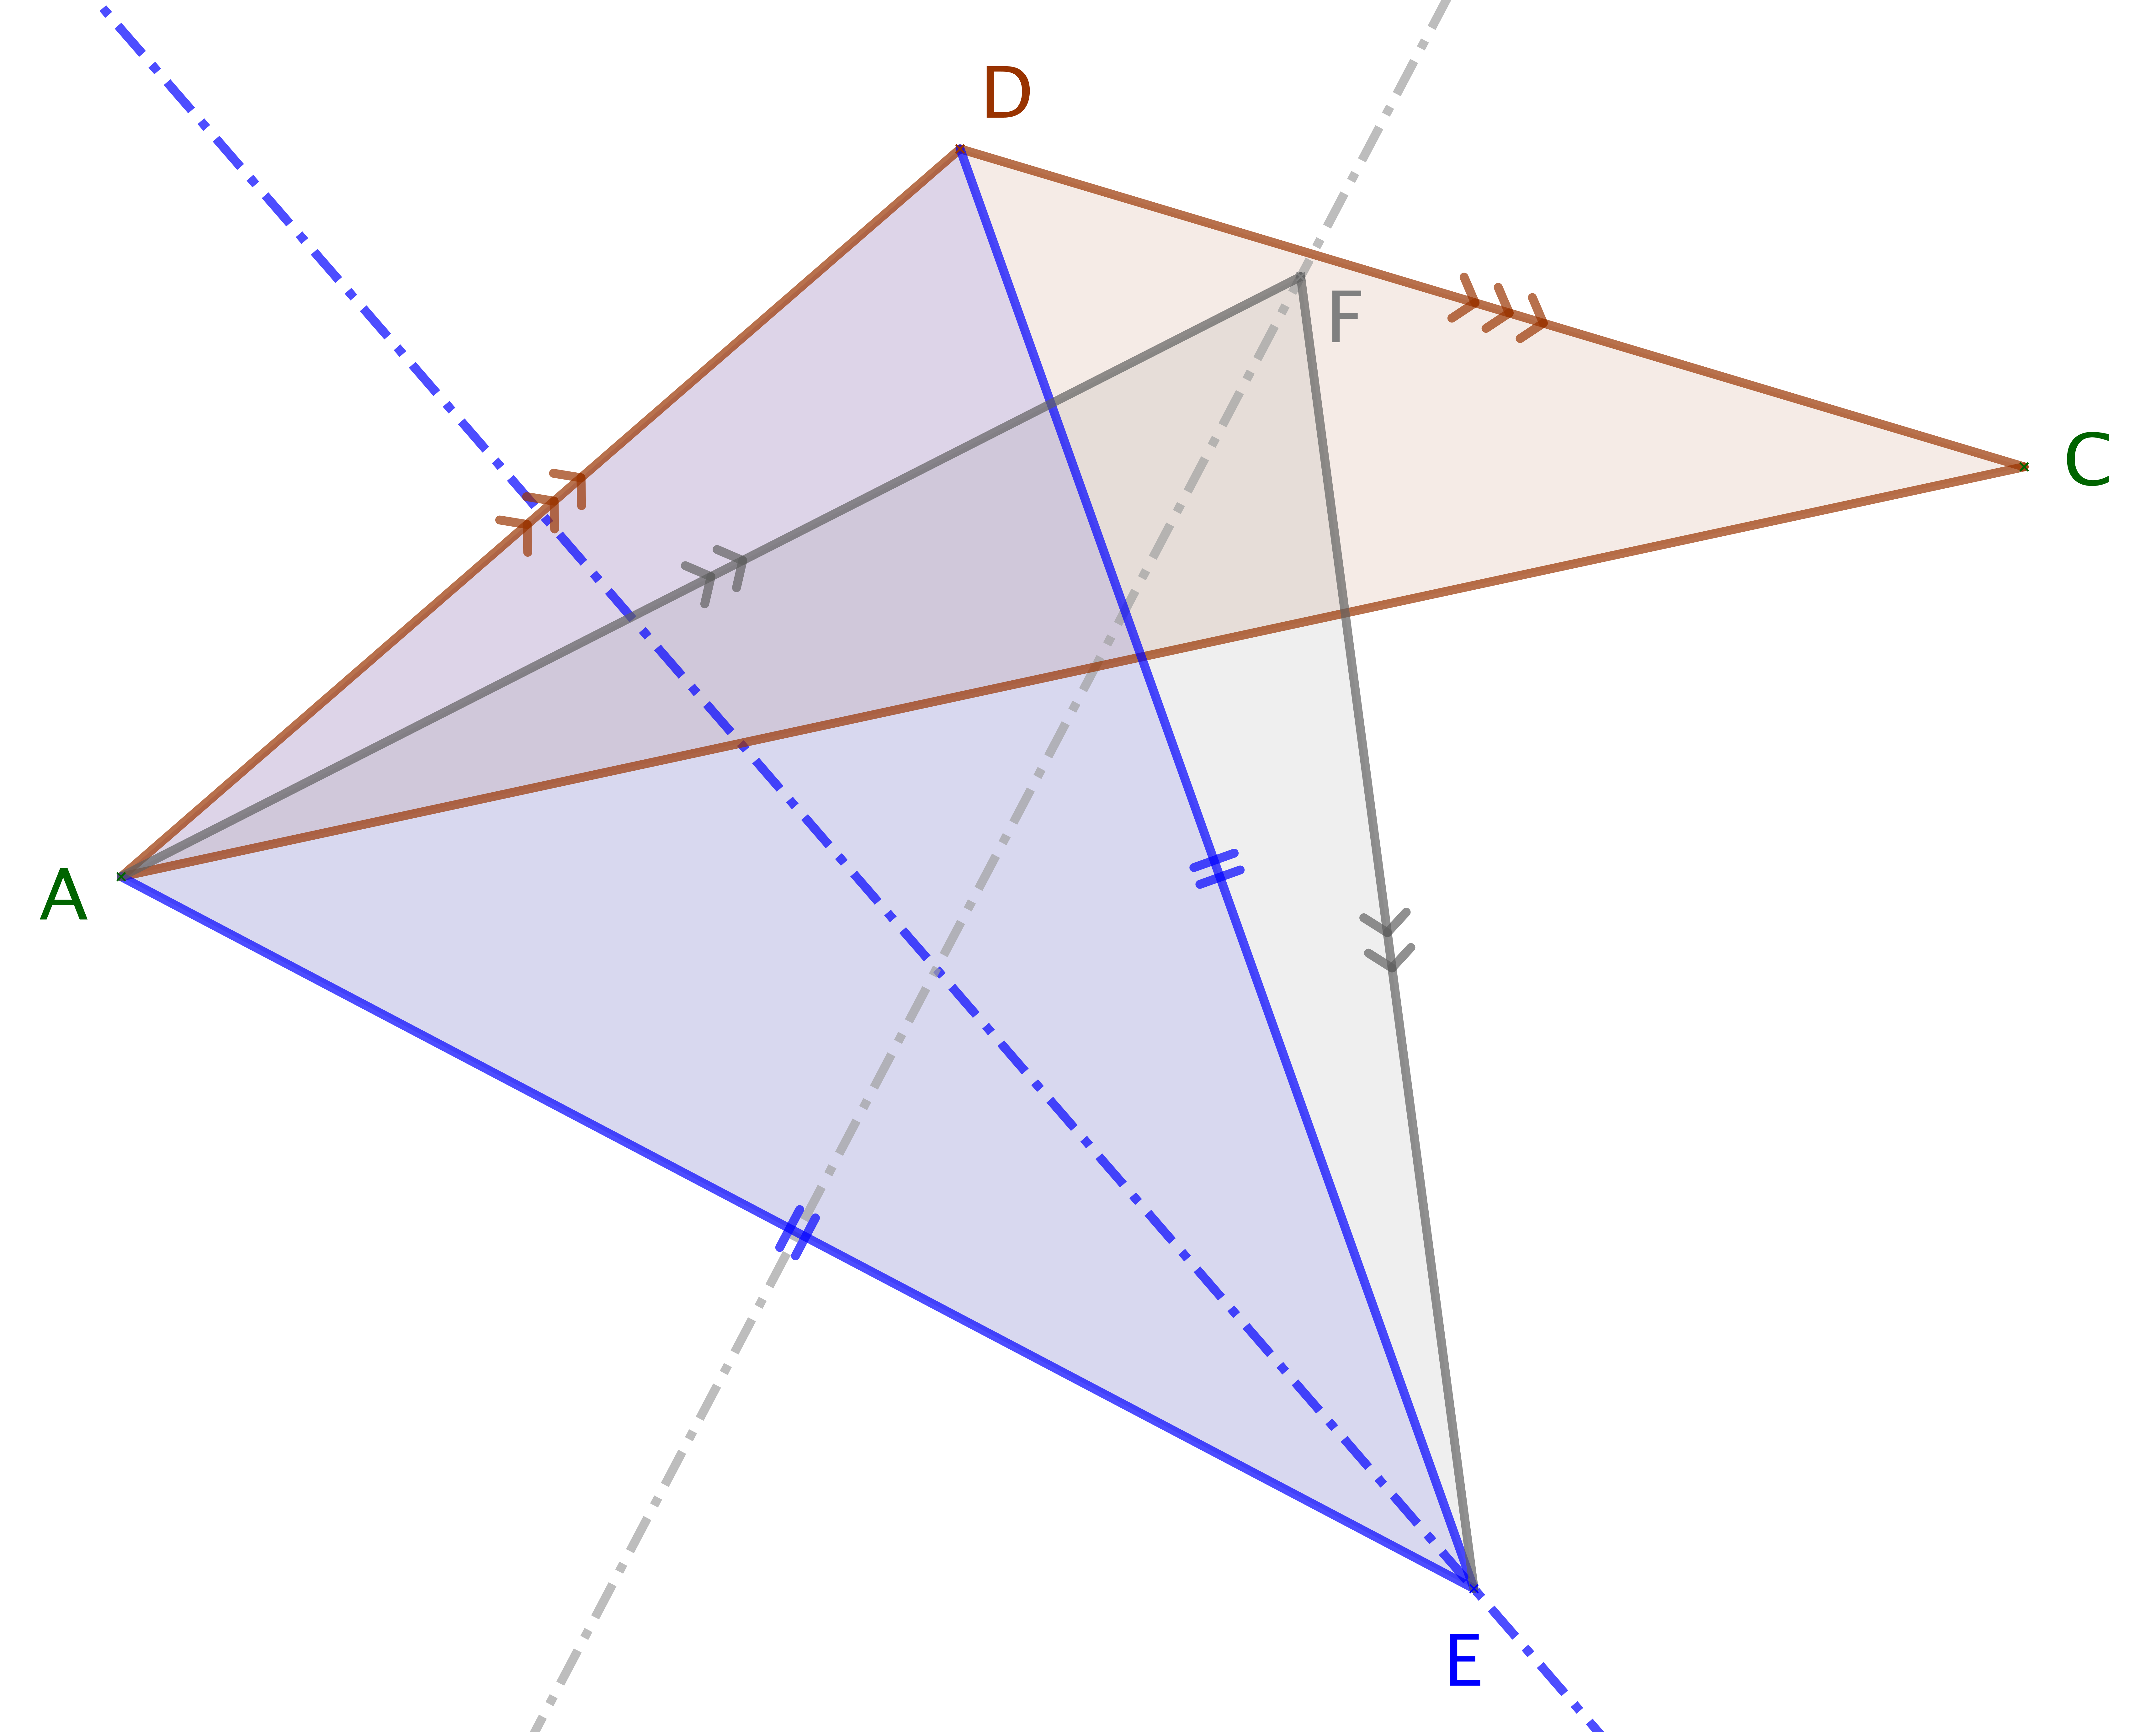
\includegraphics[scale=.4]{content/triangle-gene/triangle-proof.png}
	\end{center} 
	
	
	Voici ce que nous pouvons affirmer.
	%
	\begin{enumerate}
		\item Considérons $ACD$ isocèle en $D$ tel que $AC > AD$.
		%
		Comme $AC + AD + DC = p$, nous avons $AC > \frac13p > AD$.
		Dès lors, on doit avoir ensuite  $AD < \frac13p < AE$, car $AD + DE + AE = p$ et $AD = AE$.


		\item Considérons $ADE$ isocèle en $E$ tel que $AD < AE$ en oubliant le point précédent.
		%
		Comme $AD + DE + AE = p$, nous avons $AD < \frac13p < AE$.
		Dès lors, on doit avoir ensuite  $AE > \frac13p > AF$, car $AE + AF + EF = p$ et $AF = EF$.


		\item Les deux points précédents démontrent que notre procédé n'arrivera jamais en un nombre fini d'étapes à un triangle équilatéral si l'on part d'un triangle isocèle non équilatéral.%
		\footnote{
			Et plus généralement si le procédé ne commence pas avec une base de longueur $\frac13 p$.
		}


		\item Nous devons quantifier les écarts à la mesure \og \emph{limite} \fg\ $p^{\,\prime} = \frac13 p$. 
		%
		\begin{itemize}
			\item Dans $ADC$, posant $AD = p^{\,\prime} - \epsilon$, nous avons $AC = p^{\,\prime} + 2 \epsilon$.

			\item Dans $ADE$, posant $AE = p^{\,\prime} + \epsilon^{\,\prime}$, nous avons $AD = p^{\,\prime} - 2 \epsilon^{\,\prime}$.

			\item Donc $\epsilon^{\,\prime} = \frac12 \epsilon$.
		\end{itemize}
		
		\noindent
		Nous avons donc une convergence exponentielle des longueurs des côtés vers $p^{\,\prime} = \frac13 p$. Et tout ceci via de la géométrie et de l'analyse élémentaires!
	\end{enumerate}
\end{proof}


% ----------------------- %


\begin{remark}
	La preuve élémentaire classique commence par noter que si $ABC$ n'est pas équilatéral, en particulier il n'est pas isocèle en $A$, donc, selon le fait \ref{tri-one-side-fixed}, il existe un triangle isocèle de base $[BC]$, de même périmètre et d'aire strictement plus grande.
	Ceci nous prouve qu'un triangle maximisant l'aire à périmètre fixé ne peut être qu'équilatéral. 
	Cette condition nécessaire est-elle suffisante? Ce sera vrai si nous savons qu'au moins un triangle maximisant l'aire à périmètre fixé existe, puisque, dans ce cas, un tel triangle ne pourra être qu'équilatéral.%
	\footnote{
		Sans cette existence, il se pourrait, par exemple, que le triangle équilatéral soit à part, et que les autres aient des aires augmentant indéfiniment de leur côté, sans mauvais jeu de mots, en dépassant celle du triangle équilatéral qui serait une sorte de maximum local isolé.
	}
	Nous voilà obligé de faire appel aux techniques d'analyse.
	%
	\begin{itemize}
		\item On munit le plan d'un repère orthonormé $\pvaxes{O | i | j}$. 

		\item Les triangles $ABC$ tels que $\perim{ABC} = p$ sont représentés en posant $A\coord{0 | 0}$, $B\coord{AB | 0}$ et $C\coord{x_C | y_C}$ avec $y_C \geq 0$. Un triangle peut donc avoir trois représentations, mais peu importe.
		De plus, on accepte les triangles dégénérés pour lesquels nous avons $y_C = 0$ dans notre représentation.
		Nous notons alors $\setproba{T} \subset \RR^3$ l'ensemble des triplets $\coord{x_B | x_C | y_C}$ ainsi obtenus.

		\item Il est facile de justifier que $\setproba{T}$ est fermé dans $\RR^3$.
		De plus, $\setproba{T}$ est borné car $x_B$, $x_C$ et $y_C$ le sont.
		En résumé, $\setproba{T}$ est un compact de $\RR^3$.

		\item La fonction $s: \coord{x_B | x_C | y_C} \in \setproba{T} \mapsto \num{.5} x_B y_C \in \RRp$ est la fonction aire des triangles représentés.
		Par continuité et compacité, on sait que $s$ admet un maximum sur $\setproba{T}$. Mission accomplie!
	\end{itemize}
\end{remark}


% ----------------------- %


\begin{remark}
	La formule de Héron donne qu'un triangle de côtés $a$, $b$ et $c$, et de demi-périmètre $s = \num{.5} p$, possède une aire égale à $\sqrt{s(s - a)(s - b)(s - c)}$.
	La comparaison des moyennes géométriques et arithmétiques d'ordre $3$ nous donne alors une solution algébrique efficace, puisque de
	$\sqrt[3]{(s - a)(s - b)(s - c)} \leq \frac13 \big( (s - a) + (s - b) + (s - c) \big)$,
	nous déduisons
	$s(s - a)(s - b)(s - c) \leq \frac{1}{27} s^4$,
	puis
	$\sqrt{s(s - a)(s - b)(s - c)} \leq \frac{p^2}{12 \sqrt{3}}$
	où $\frac{p^2}{12 \sqrt{3}}$ est l'aire du triangle équilatéral de périmètre $p$.
\end{remark}


% ----------------------- %


\begin{remark} \label{constrained-extrema}
	L'aire d'un triangle étant positive ou nulle, nous pouvons chercher à maximiser son carré
	$f(a;b;c) = s(s - a)(s - b)(s - c)$,
%	          = \frac{1}{16} (a + b + c)(b + c - a)(a + c - b)(a + b - c)$,
	sous la contrainte $2s = a + b + c$ où $s > 0$ est constant.
	Notant $g(a;b;c) = a + b + c - 2 s$, la contrainte s'écrit $g(a;b;c) = 0$.
	%
	\begin{itemize}
		\item Si un extremum existe,
    	$\exists \lambda \in \RR$ tel que
    	$\pder[i]{f}{a}{1} = \lambda \pder[i]{g}{a}{1}$,
    	$\pder[i]{f}{b}{1} = \lambda \pder[i]{g}{b}{1}$ et
    	$\pder[i]{f}{c}{1} = \lambda \pder[i]{g}{c}{1}$
		d'après la méthode des extrema liés.

		\item Donc
		$- s(s - b)(s - c) = - s(s - a)(s - c) = - s(s - a)(s - b)$,
		et par conséquent
		$(s - b)(s - c) = (s - a)(s - c) = (s - a)(s - b)$.

		\item Les cas $s = a$, $s = b$ et $s = c$ donnent $f(a;b;c) = 0$.

		\item Le cas $\big[ s \neq a, s \neq b \text{ et } s \neq c \big]$ n'est envisageable que si $a = b = c = \frac{p}{3}$, ceci impliquant $f(a;b;c) = \frac{1}{16} p \big( \frac{p}{3} \big)^3 = \big( \frac{p^2}{12 \sqrt{3}} \big)^2 > 0$.

		\item En résumé, l'existence d'un maximum implique que ce maximum corresponde au cas du triangle équilatéral.

		\item Il reste à démontrer qu'un tel maximum existe pour pouvoir conclure: ceci est facile à justifier en considérant l'ensemble compact $\intervalC{0}{2s}^3$ de $\RR^3$.
	\end{itemize}
\end{remark}
